\Subsection{Колмогоровская модель теории вероятности}

\begin{definition}
    $(\Omega, \mathcal{F}, P)$ - вероятностное пространство.

    $\Omega$ - множество или пространство элементарных исходов.

    $\mathcal{F}$ - $\sigma$-алгебра подмножеств $\Omega$. Элементы $\mathcal{F}$ - случайный события.

    $P$ - мера на $\mathcal{F}$ с условием $P(\Omega) = 1$.

    \begin{remark}
        Если $\Omega$ не более чем счётно, то можно взять $\mathcal{F} = 2^{\Omega}$
    \end{remark}
\end{definition}

\begin{definition}
    Условная вероятность. $A$ - событие, такое, что $P(A) > 0$.
    Тогда $P(B | A) = \frac{P(B \cap A)}{P(A)}$, где $A, B \in \mathcal{F}$.
\end{definition}

\begin{definition}
    Независимые события $A$ и $B$. Если $P(A \cap B) = P(A) \cdot P(B)$
\end{definition}

\begin{definition}
    Независимость в совокупности $A_1, A_2 \ldots A_n$. $P(A_{i_1} \cap \ldots \cap A_{i_k}) = P(A_{i_1}) \cdot \ldots \cdot P({A_{i_k}})$
    для всевозможных наборов индексов.
\end{definition}

\begin{definition}
    Последовательность событий $A_1, A_2 \ldots $ независимы - любой конечный набор событий
    независим в совокупности.
\end{definition}

\begin{lemma}
    \textbf{Бореля-Кантелли}

    $A_1, A_2, \ldots$ случайные события.

    \begin{enumerate}
        \item {
            Если $\sum_{n = 1}^{\infty} P(A_n) < +\infty$, то вероятность, что случилось бесконечное число из них равна 0.
        }
        \item {
            Если $A_1, A_2, \ldots$ независимы и $\sum_{n = 1}^{\infty} P(A_n) = +\infty$, тогда

            $P(\text{случилось бесконечное число из $A_n$}) = 1$.
        }
    \end{enumerate}
\end{lemma}

\begin{proof}
    $B = \bigcap_{n = 1}^{\infty} \bigcup_{k = n}^{\infty} A_k$ - это переформулировка события из условия в терминах множеств.

    $\omega \in B \Longleftrightarrow \omega \in \bigcup_{k = n}^{\infty} A_k \ \forall n \Longleftrightarrow w \in A_k$ для бесконечного количества индексов $k$.

    Док-во этого факта:

    \begin{enumerate}
        \item $\Leftarrow:$ Лежит в каждом объединении, значит лежит в $B$.
        \item $\Rightarrow:$ $\omega$ лежит в пересечении. Пусть лежит в конечном - возьмём самый большой номер и получим противоречие.
    \end{enumerate}

    Док-во теоремы:

    \begin{enumerate}
        \item {
            Хотим доказать, что $P(B) = 0$

            $B \subset \bigcup_{k = n}^{\infty} A_k \Rightarrow P(B) \leqslant P(\bigcup_{k = n}^{\infty} A_k) \leqslant \sum_{k = n}^{\infty} P(A_k)$ - это хвост сходящегося ряда, а он стремится к нулю.

        }
        \item {
            Давайте смотреть на $\bar{A_1}, \bar{A_2}, \ldots$ - независимые события.

            $P(\bigcap_{k = 1}^n \bar{A_k}) \overbrace{=}^{\text{независимость}} \prod_{k = 1}^{n} P(\bar{A_k}) \to_{n \to \infty} \prod_{k = 1}^{\infty}  P(\bar{A_k}) = \prod_{k = 1}^{\infty}  (1 - P(A_k))$

            А ещё $P(\bigcap_{k = 1}^n \bar{A_k}) \rightarrow P(\bigcap_{k = 1}^\infty \bar{A_k})$, так как множества вложены в друг друга и есть монотонность меры.

            \hfill \smallbreak

            Значит $P(\bigcap_{k = n}^\infty \bar{A_k}) = \prod_{k = n}^{\infty}  (1 - P(A_k)) \overset{\text{логарифмируем}} {\Longleftrightarrow}
            \ln P(\bigcap_{k = n}^\infty \bar{A_k}) = \\ = \sum_{k = n}^{\infty} \ln (1 - P(A_k)) \overset{\ln (1 - t) \leqslant -t}{\leqslant}
            \sum_{k = n}^{\infty} (-P(A_k)) = -\infty$ - хвост расходящегося ряда.

            А значит мы логарифмировали $0 \Rightarrow P(\bigcap_{k = n}^{\infty} \bar{A_k}) = 0 \Rightarrow P(\bigcup_{n=1}^{\infty} \bigcap_{k = n}^{\infty} \bar{A}_k) = 0 \Rightarrow P(\bar{B}) = 0 \overset{(*)}{\Rightarrow} P(B) = 1$

            $(*) \, \overline{\bigcup_{n=1}^{\infty} \bigcap_{k = n}^{\infty} \bar{A}_k} = \bigcap_{n=1}^{\infty} \bigcup_{k=n}^{\infty} A_k = B$
        }
    \end{enumerate}
\end{proof}

\begin{theorem}
    \textbf{Закон нуля и единицы}

    Если $A_1, A_2 \ldots$ независимы, то $P(B) = 0$ или $P(B) = 1$. При $B = \bigcap_{n = 1}^{\infty} \bigcup_{k = n}^{\infty} A_k$.
\end{theorem}

\begin{example}
    Испытания Бернулли, успех с вероятностью $p$,

    $P(\text{ОРО встречается бесконечное число раз}) = \ ?$.

    $A_n = $ случилось $\text{ОРО}$ на позициях $n, n + 1, n + 2$.

    Тогда $A_1, A_4, A_7, \ldots$ независимы. $P(A_j) = pqp = p^2 q > 0$.

    Лемма Бореля-Кантелли говорит: бесконечное кол-во $A_{3k + 1}$ случится, если $\sum_{k=1}^{\infty} {P(A_{3k + 1})} = +\infty \implies P(\text{ОРО встречается бесконечное число раз}) = 1$.
\end{example}

\Subsection{Случайные величины}

\begin{definition}
    $(\Omega, \mathcal{F}, P)$ - вероятностное пространство.

    $\xi: \Omega \to \mathbb{R}$ - случайная величина, если
    это измеримая функция.
\end{definition}

\begin{definition}
    Распределение случайное величины

    $P_{\xi}$ - вероятностная мера на борелевских подмножествах
    $\mathbb{R}$

    $A$ -- борелевское мн-во, $P_{\xi}(A) = P(\omega \in \Omega \ : \ \xi(\omega) \in A)$
\end{definition}

\begin{definition}
    Случаный величины $\xi$ и $\eta$ одинаково распределены, если
    $P_{\xi} = P_{\eta}$
\end{definition}

\begin{remark}
    $P_{\xi}$ однозначно определяются своими значениями на ячейках.

    $P_{\xi} (a, b] = P_{\xi} (-\infty, b] - P_{\xi} (-\infty, a] =
    P(\xi \leqslant b) - P(\xi \leqslant a)$
\end{remark}

\begin{definition}
    Функция распределения случайной величины

    $F_{\xi} (x) = P(\xi \leqslant x)$
\end{definition}

\begin{properties}
    \begin{enumerate}
        \item {
        Функция распределения однозначно определяет распределение
        случайной величины.

        \begin{proof}
            Функция распределения однозначно задаёт значения на ячейках
        \end{proof}
        }
        \item {
            $0 \leqslant F_{\xi}(x) \leqslant 1 \, \forall x \in \mathbb{R}$
        }

        \item {
            $\lim_{x \to -\infty} F_{\xi} (x) = 0$

            $\lim_{x \to +\infty} F_{\xi} (x) = 1$

            \begin{proof}
                берём $x_n \to -\infty, A_n = \{ \xi \leqslant x_n \} $
                Тогда $A_{n + 1} \subset A_n$. Тогда $\lim_{n \to \infty} P(A_n) =
                P(\bigcap_{n = 1}^{\infty} A_n) = P(\emptyset) = 0$
            \end{proof}
        }
        \item {
            $F_{\xi}$ монотонно возрастает
        }
        \item {
            Непрерывность справа: $\lim_{y \to x+} F_{\xi} (y) = F_{\xi} (x)$

            \begin{proof}
                берём $y_n$ убывающие и $y_n \to x$.
                Тогда $A_n = \{ \xi \leqslant y_n \}$. $A_{n + 1} \subset A_n$.
                А тогда $\lim P(A_n) = P(\bigcap_{n = 1}^{\infty} A_n) = P(\xi \leqslant x) = F_{\xi} (x)$.
                Но с другой стороны $\lim P(A_n) = \lim P(\xi \leqslant y_n) = \lim F_{\xi} (y_n)$
            \end{proof}

            }
        \item {
            $\lim_{y \to x-} F_{\xi} (y) = P(\xi < x)$

            \begin{proof}
                берём $y_n$ возрастающие и
                $y_n \to x$. $B_n = \{ \xi \leqslant y_n \}$ и $B_{n} \subset B_{n + 1}$.
                $\lim P(B_n) = P(\bigcup B_n) = P(\xi < x)$. Но с другой стороны
                $\lim P(B_n) = \lim F_{\xi} (y_n)$
            \end{proof}
        }
        \item {
            $F_{\xi + a} (x) = F_{\xi} (x - a)$

            \begin{proof}
                $\{ \xi + a \leqslant x \} = \{ \xi \leqslant x - a \}$
            \end{proof}
        }
        \item {
            $F_{c\xi} = F_{\xi} (\frac{x}{c})$

            \begin{proof}
                $\{ c\xi \leqslant x \} =  \{ \xi \leqslant \frac{x}{c} \}$
            \end{proof}
        }
    \end{enumerate}

    \begin{remark}
        Фукнция, обладающая свойствами 3, 4, 5 - это фукнция распределения
        некоторой случайной величины.

        \begin{proof}
            пусть $g$ - такая функция. Тогда $\nu_g (a, b] = g(b) - g(a)$. $\Omega = \mathbb{R}$, $\mathcal{F}$ - измеримо по Лебегу, случайная величина $\xi (w) = w$. Тогда $F_{\xi} = g$
        \end{proof}
    \end{remark}

\end{properties}

\begin{definition}
    Случайная величина имеет дискретное распределение, если её
    множество значений не более чем счётное.

    \begin{remark}
        \begin{enumerate}
            \item { $\xi \to \{y_1, y_2, \ldots \}$

            Если $x \neq y_k$, то $P(\xi = x) = 0$, т.е. $P_{\xi}(\{ x \}) = 0$
            }

            \item { $P_{\xi} (A) = \sum_{k : y_k \in A} P(\xi = y_k)$. Тут счётное
            число слагаемых, поэтому сумма корректно определена.

            Распределение однозначно определяется набором вероятностей $P(\xi = y_k)$
            }
            \item {
                $F_{\xi} (x) = \sum_{k : y_k \leqslant x} P(\xi = y_k)$
            }
        \end{enumerate}
    \end{remark}
\end{definition}

\begin{definition}
    Случайная величина имеет непрерывное распределение, если
    $\forall x\in \mathbb{R}: P(\xi = x) = 0$

    \begin{remark}
        \begin{enumerate}
            \item {
                $\xi$ -- имеет непрерывное распределение $\Longleftrightarrow$ $F_{\xi}$ непрерывна во всех точках.

                $P(\xi < x) = \lim_{y\rightarrow x-}P(\xi \leq y) = \lim_{y\rightarrow x-} F_{\xi}(y)$

                $0 = P(\xi = x) = P(\xi \leq x) - P(\xi < x) = F_{\xi}(x) - \lim_{y\rightarrow x-}F_{\xi}(y) \Rightarrow F_{\xi}(x) = \lim_{y\rightarrow x-}F_{\xi}(y)$
            }
            \item {
                Непрерывные распределения бывают не очень хорошими, например
                Канторова лестница.
            }
        \end{enumerate}
    \end{remark}
\end{definition}

\begin{definition}
    Случайная величина имеет абсолютно непрерывное распределение, если
    существует $p_{\xi} (t) \geqslant 0$, измеримая, т.ч. $F_{\xi} (x) =
    \int_{-\infty}^x p_{\xi} (t) \, dt$ ($p_{\xi}(t)$ -- плотность распределения).
\end{definition}

\begin{properties}
    \begin{enumerate}
        \item {
            $A \subset \mathbb{R}$ -- борелевское, то $P_{\xi} (A) = \int_{A} p_{\xi} (t) \, dt$

            \begin{proof}
                слева мера и справа написаны меры. На лучах они совпадают по определению, значит совпадают
                на ячейках, а значит и совпадают везде
            \end{proof}

            $P_{\xi} (a, b] = F_{\xi} (b) - F_{\xi} (a) = \int_{a}^b p_{\xi} (t) \, dt$
        }
        \item {
            $\int_{-\infty}^{+\infty} p_{\xi} (t) \, dt = 1$
        }
        \item {
            $p_{\xi}$ определена однозначно с точностью до почти везде (из теории меры)
        }
        \item {
            $F_{\xi}$ почти везде диффиренцируема и $F_{\xi}' (x) = p_{\xi} (x)$

            \begin{proof}
                без доказательства
            \end{proof}
        }
    \end{enumerate}
\end{properties}

\begin{example}
    \textbf{Вероятностные распределения}

    \begin{enumerate}
        \item {
            Биномиальное распределение: $\xi \sim Binom(p, n), 0 < p < 1$

            $\xi : \Omega \to \{ 0, 1, \ldots n \}$. $P(\xi = k) = \binom{n}{k} p^k (1 - p)^{n - k}$
        }
        \item {
            Распределение Пуассона: $\xi \sim Poisson(\lambda), \lambda > 0$.

            $\xi : \Omega \to \{ 0, 1, \ldots \}$. $P(\xi = k) = \frac{\lambda^k}{k!}e^{-\lambda}$
        }
        \item {
            Геометрическое распределение: $\xi \sim Geom(p), 0 < p < 1$.

            $\xi : \Omega \to \{ 1, 2, \ldots \}$. $P(\xi = k) = p(1 - p)^{k - 1}$.
        }
        \item {
            Дискретное равномерное распределение: %$\xi \sim U(\ldots)$

            $\xi : \Omega \to \{ 1, 2, \ldots n \}$. $P(\xi = k) = \frac{1}{n}$
        }
        \item {
            Непрерывно равномерное распределение: $\xi \sim U([a, b])$

            $\xi : \Omega \to [a, b]$. $p_{\xi}(t) = \frac{1}{b - a} \cdot \mathds{1}_{[a, b]} (t)$
        }
        \item {
            Нормальное распределение: $\xi \sim \mathcal{N} (a, \sigma^2), a \in \mathbb{R}, \sigma > 0$

            $\xi : \Omega \to \mathbb{R}$. $p_{\xi}(t) = \frac{1}{\sqrt{2\pi} \cdot \sigma} e^{-\frac{(t - a)^2}{2\sigma^2}}$

            Стандартное нормальное распределение: $\mathcal{N} (0, 1)$
        }
        \item {
            Экспонециальное распределение: $\xi \sim Exp(\lambda), \lambda > 0$.

            $\xi : \Omega \to [0, +\infty]$. $p_{\xi}(t) = \begin{cases}
                \lambda e^{-\lambda t}, \text{ при } t \geqslant 0 \\
                0, \text{ в других точках}
            \end{cases}$
        }
    \end{enumerate}

    \begin{remark}
        \begin{enumerate}
            \item {
                $\Phi (x) = \frac{1}{\sqrt{2 \pi}} \int_{-\infty}^{x} e^{-\frac{t^2}{2}} \, dt$.

                На самом деле это функция распределения стандартной нормальной случайной величины.
            }
            \item {
                Если $\nu \sim \mathcal{N}(0, 1)$, то $\xi = \sigma \nu + a$. $\xi \sim \mathcal{N}(a, \sigma^2)$

                $F_{\xi} (x) = P(\sigma \nu + a \leqslant x) = P(\nu \leqslant \frac{x - a}{\sigma}) = \frac{1}{\sqrt{2 \pi}}
                \int_{-\infty}^{\frac{x - a}{\sigma}} e^{-\frac{t^2}{2}} \, dt$

                Замена $t = \frac{s - a}{\sigma}$. Тогда $dt = \frac{ds}{\sigma}$

                Тогда: $\frac{1}{\sqrt{2 \pi}}
                \int_{-\infty}^{\frac{x - a}{\sigma}} e^{-\frac{t^2}{2}} \, dt = \frac{1}{\sqrt{2\pi} \sigma}
                \int_{-\infty}^{x} e^{-\frac{(s - a)^2}{2\sigma^2}} \, ds$
            }
        \end{enumerate}

    \end{remark}
\end{example}

\Subsection{Совместное распределение}

\begin{definition}
    Совместное (многомерное) распределение.

    $\bar{\xi} = (\xi_1, \xi_2, \ldots, \xi_n) : \Omega \to \mathbb{R}^n$

    $P_{\bar{\xi}} (A) = P(\bar{\xi} \in A)$, где $A$ - борелевское подмножество $\mathbb{R}^n$

    \begin{remark}
        $P_{\bar{\xi}}$ однозначно определяет распределение $P_{\xi_k}$, но не наоборот

        \begin{example}
            $\xi, \eta : \Omega \to \{ 0, 1 \}$  с равными вероятностями.

            Если это были независимые подбрасывания: $(\xi, \eta) : \Omega \to
            \{ (0, 0), (0, 1), (1, 0), (1, 1) \}$  с равными вероятностями.

            Если $\xi = \eta$, то $(\xi, \eta) : \Omega \to \{ (0, 0), (1, 1) \}$.

            То есть получили 2 разных совместных распределения, при это координатное распределение только одно

        \end{example}
    \end{remark}
\end{definition}

\begin{definition}
    Случайные величины $\xi_1, \xi_2 \ldots \xi_n$ независимы, если для любых
    борелевских подмножеств $A_1, A_2 \ldots A_n \subset \mathbb{R}$, события
    $\{ \xi_1 \in A_1 \}, \ldots, \{ \xi_n \in A_n \}$ независимы

    \begin{remark}
        $P(\xi_1 \in A_1, \ldots, \xi_n \in A_n) = P(\xi_1 \in A_1) \cdot \ldots \cdot P(\xi_n \in A_n)$
    \end{remark}
\end{definition}

\begin{theorem}
    $\xi_1, \xi_2 \ldots \xi_n$ независимы $\Longleftrightarrow P_{\bar{\xi}} = P_{\xi_1} \times \ldots \times P_{\xi_n}$
\end{theorem}

\begin{proof}
    \begin{enumerate}
        \item $\Leftarrow$ $P(\xi_1 \in A_1, \ldots, \xi_n \in A_n) = P_{\xi_1, \ldots, \xi_n} (A_1 \times \ldots \times A_n) = P_{\xi_1} (A_1) \cdot \ldots \cdot P_{\xi_n} (A_n)$
        \item {
            $\Rightarrow$. Достаточно проверить совпадение на ячейках, то есть, что $P(\bar{\xi} \in (a, b]) = P_{\xi_1} (a_1, b_1] \cdot
            \ldots \cdot P_{\xi_n} (a_n, b_n]$. А это просто определение независимости.
        }
    \end{enumerate}
\end{proof}

\begin{definition}
    Совместная (многомерная) функция распределения.

    $\bar{\xi} = (\xi_1 \ldots \xi_n)$. $F_{\bar{\xi}} : \mathbb{R}^n \to \mathbb{R}$. и
    $F_{\bar{\xi}} (\bar{x}) = P(\xi_1 \leqslant x_1,  \ldots, \xi_n \leqslant x_n) $
\end{definition}

\begin{properties}
    \begin{enumerate}
        \item {
            $0 \leqslant F_{\bar{\xi}} \leqslant 1$
        }
        \item {
            Монотонно возрастает по каждой координате
        }
        \item {
            $\lim_{x_i \to -\infty} F_{\bar{\xi}} (\bar{x}) = 0$

            $\lim_{x_1, \ldots, x_n \to +\infty} F_{\bar{\xi}} (\bar{x}) = 1$
        }
        \item {
            $\lim_{x_i \to +\infty} F_{\bar{\xi}} (\bar{x}) = F_{\xi_1, \ldots, \xi_{i - 1}, \xi_{i + 1}, .., \xi_n}(x_1, .., x_{i-1}, x_{i+1}, .., x_n)$
        }
    \end{enumerate}
\end{properties}

\begin{definition}
    Совместная плотность $p_{\bar{\xi}} (\bar{t})$ - неотрицательная измеримая функция, такая, что $F_{\bar{\xi}} (\bar{\xi}) = \int_{-\infty}^{x_1} \ldots \int_{-\infty}^{x_n} p_{\bar{\xi}} (\bar{t}) \, dt_n \ldots dt_1$
\end{definition}

\begin{theorem}
    $\xi_1 \ldots \xi_n$ независимы $\Longleftrightarrow F_{\bar{\xi}} (\bar{x}) = F_{\xi_1} (x_1) \cdot \ldots \cdot F_{\xi_n} (x_n), \ \forall \bar{x} \in \mathbb{R}^n$
\end{theorem}

\begin{proof}
    \begin{enumerate}
        \item {
            Докажем $\Rightarrow$. Независимость $\Rightarrow (*) P_{\bar{\xi}} = P_{\xi_1} \times \ldots \times P_{\xi_n} \Rightarrow
            P_{\bar{\xi}} ((-\infty, x_1] \times \ldots \times (-\infty, x_n]) = P_{\xi_1} (-\infty, x_1] \cdot \ldots \cdot P_{\xi_n} (-\infty, x_n]$
        }
        \item {
            Хотим проверить совпадение на ячейках, чтобы доказать $(*)$ ещё и в другую сторону (приведем выкладки для $n=2$, для больших $n$ рассуждения не меняются).

            \begin{center}
                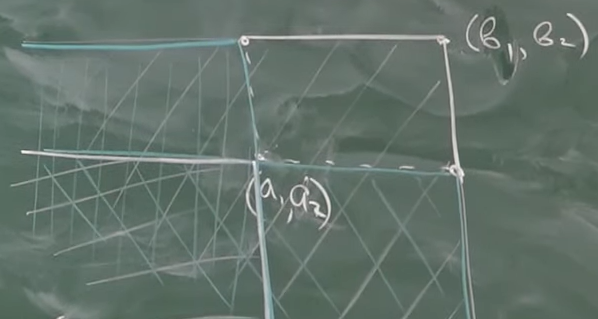
\includegraphics[width=10cm]{assets/02-general-prob-theory/arbitrary-value-independence.png}
            \end{center}

            $P_{\bar{\xi}}((a_1, b_1] \times (a_2, b_2]) = F_{\bar{\xi}} (b_1, b_2)  + F_{\bar{\xi}} (a_1, a_2) - F_{\bar{\xi}} (a_1, b_2) - F_{\bar{\xi}} (a_2, b_1) =$

            $= (F_{\xi_1} (b_1) - F_{\xi_1}(a_1)) \cdot (F_{\xi_2}(b_2) - F_{\xi_2}(a_2)) = P_{\xi_1} (a_1, b_1] \cdot P_{\xi_2}(a_2, b_2]$
        }
    \end{enumerate}
\end{proof}

\begin{consequence}
    $\xi_1 \ldots \xi_n$ - абсолютно непрерывные случайные величины. Тогда
    $\xi_1 \ldots \xi_n$ независимы $\Longleftrightarrow p_{\bar{\xi}} (\bar{t}) = p_{\xi_1} (t_1) \cdot \ldots \cdot p_{\xi_n}(t_n)$

    В частности, в случае независимости $\bar{\xi}$ абсолютно непрерывна.
\end{consequence}

\begin{proof}
    \begin{enumerate}
        \item {
            Докажем $\Rightarrow$.

            Независимость $\Rightarrow F_{\bar{\xi}} (\bar{x}) = F_{\xi_1} (x_1) \cdot \ldots \cdot F_{\xi_n} (x_n) =
            \int_{-\infty}^{x_1} p_{\xi_1} (t_1) \, dt_1 \cdot \ldots \cdot \int_{-\infty}^{x_n} p_{\xi_n} (t_n) \, dt_n =
            \int_{-\infty}^{x_1} \ldots \int_{-\infty}^{x_n} p_{\xi_1} (t_1) \ldots p_{\xi_n} (t_n) \, dt_n \ldots dt_1$.

            Запихали всё под один интеграл, то что под интегралом и есть совместная плотность.
        }
        \item {
            Докажем $\Leftarrow$.

            Просто проинтегрируем равенство.

            $\int_{-\infty}^{x_1} \ldots \int_{-\infty}^{x_n} p_{\bar{\xi}} (\bar{t}) \, dt_n \ldots dt_1 =
            \int_{-\infty}^{x_1} \ldots \int_{-\infty}^{x_n} p_{\xi_1} (t_1) \ldots p_{\xi_n} (t_n) \, dt_n \ldots dt_1 =$

            $\underbrace{=}_{\text{по т. Тонелли можно выносить интегралы}} F_{\xi_1} (x_1) \cdot \ldots \cdot F_{\xi_n} (x_n)$

            т. Тонелли можно использовать, так как мы интегрируем неотрицательную функцию.
        }
    \end{enumerate}
\end{proof}

\begin{remark}
    Напоминание.

    Свертка последовательностей: $\{a_n\}, \{b_n\}$ это $\{c_n\}$, такая что $c_n = a_0 b_n + a_1 b_{n - 1} + \ldots + a_n b_0$.

    Мотивировка: $\left(\sum_{n=0}^{\infty}a_n z^n\right) \cdot \left(\sum_{n = 0}^{\infty} b_n z^n\right) = \sum_{n=0}^{\infty} c_n z^n$  (при наличии хоть каких-нибудь кругов сходимости у обоих рядов).
\end{remark}

\begin{remark}
    \textbf{Свертки мер}

    $\mu$ и $\nu$ - конечные меры на борелевских подмножествах $\mathbb{R}$.

    $\mu * \nu (A) = \int_{\mathbb{R}} \mu (A - x) \, d\nu (x)$ - это свертка мер, где $(A - x) := \{ a - x \ | \ a \in A \}$.

    \begin{properties}
        \textbf{Свойства свёртки}

        \begin{enumerate}
            \item {
                $\mu * \nu (A) = \int_{\mathbb{R}^2} \mathds{1}_A (x + y) d\mu (x) \, d\nu (y)$

                \begin{proof}
                    $\mu * \nu (A) = \int_{\mathbb{R}} \mu (A - x) \, d\nu (x) \overset{\mu (A - x) = \int_{\mathbb{R}} \mathds{1}_{A - x} d\mu (y) }{=}
                    \int_{\mathbb{R}} \int_{\mathbb{R}} \mathds{1}_{A - x} (y) d\mu (y) \, d\nu (x)$
                \end{proof}
            }
            \item {
                $\mu * \nu = \nu * \mu$
            }
            \item {
                $\mu_1 * \ldots * \mu_n (A) = \int_{\mathbb{R}^n} \mathds{1}_A (x_1 + \ldots + x_n) \, d\mu_1 (x_1) \ldots \, d \mu_n (x_n)$
            }
            \item {
                $(\mu_1 * \mu_2) * \mu_3 = \mu_1 * (\mu_2 * \mu_3)$
            }
            \item {
                $(\mu_1 + \mu_2) * \nu = \mu_1 * \nu + \mu_2 * \nu$
            }
            \item {
                $\delta_x$ - мера с единичной нагрузкой в точке $x$. Тогда $\mu * \delta_0 = \mu$.

                Получили линейное пространство относительно $+$ и $*$

                \begin{proof}
                    $\mu * \delta_0 (A) = \delta_0 * \mu (A) = \int_{\mathbb{R}} \delta_0 (A - x) \, d\mu (x)
                    \overset{\delta_0 = 1 \Leftrightarrow 0 \in A - x \Leftrightarrow x \in A}{=} \int_{\mathbb{R}} \mathds{1}_{A} d\mu (x) = \mu A$
                \end{proof}
            }
        \end{enumerate}
    \end{properties}
\end{remark}

\begin{theorem}
    Пусть $\mu$ и $\nu$ имеют плотности $p_{\mu}$ и $p_{\nu}$

    Тогда $\mu * \nu$ имеет плотность $p(t) = \int_{\mathbb{R}} p_{\mu} (t - s) p_{\nu} (s) \, ds$
\end{theorem}

\begin{proof}
    Возьмём функцию, определяемую этой формулой и проверим, что это плотность.

    То есть проверим, что $\int_{A} p(x) dx = \mu * \nu (A)$.

    $\int_A p(t) \, dt = \int_A \int_{\mathbb{R}} p_{\mu} (t - s) p_{\nu} (s) \, ds \, dt = \int_{\mathbb{R}}
    \int_{\mathbb{R}} \mathds{1}_A (t) p_{\mu} (t - s) p_{\nu} (s) \, ds \, dt = (*)$.

    Положим $u = t - s$. Тогда $(*) = \int_{\mathbb{R}^2} \mathds{1}_{A} (u + s) p_{\mu} (u) p_{\nu} (s) \, ds \, du =
    \int_{\mathbb{R}^2} \mathds{1}_A (u + s) \, d\nu (s) \, d \mu (u) = \mu * \nu (A)$
\end{proof}

\begin{theorem}
    Если $\xi$ и $\eta$ независимые случайный величины, то $P_{\xi + \eta} = P_{\xi} * P_{\eta}$
\end{theorem}

\begin{proof}
    Нужно взять какое-то борелевское множество и понять как устроено там распределение суммы.

    \begin{center}
        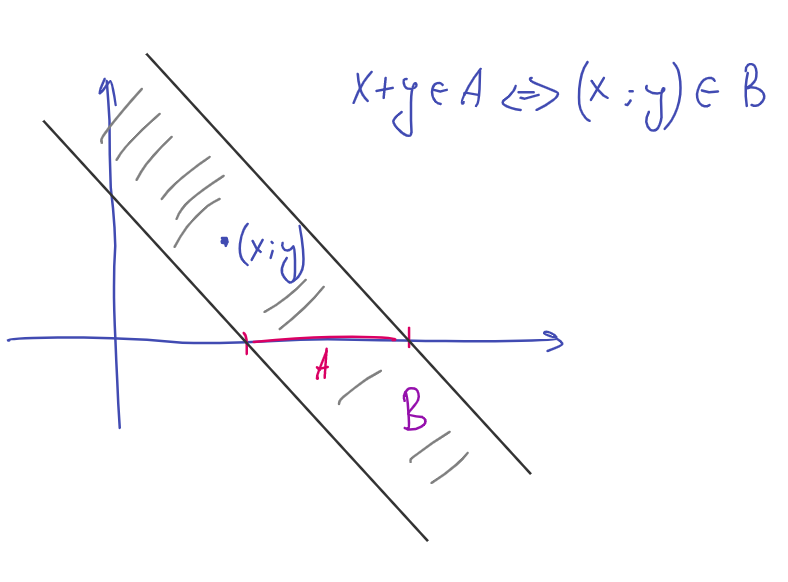
\includegraphics[width=8cm]{assets/02-general-prob-theory/new-set-B-x+y-in-A.PNG}
    \end{center}

    Пусть $B = \{ (x, y) : x + y \in A \}$

    $P_{\xi + \eta} (A) = P(\xi + \eta \in A) = P((\xi, \eta) \in B) = P_{\xi, \eta} (B) =\int_{\mathbb{R}^2} \mathds{1}_{B}(x, y) d P_{\xi, \eta}(x, y) =$

    $\underbrace{=}_{\text{т.к. $\xi$ и $\eta$ независимые}}
    \int_{\mathbb{R}^2} \mathds{1}_B (x, y) d P_{\xi} (x) \, dP_{\eta} (y) =
    \int_{\mathbb{R}^2} \mathds{1}_A (x + y) d P_{\xi} (x) \, dP_{\eta} (y) = P_{\xi} * P_{\eta} (A)$
\end{proof}

\begin{example}
    \begin{enumerate}
        \item {
            \textbf{Свертка с дисректным распределением}

            $\nu = \sum_{k = 1}^{\infty} p_k \delta_{x_k}$.

            \begin{equation}
                \delta_{x_k}(A) =
                \begin{cases}
                    1, \ x \in A \\
                    0, \ otherwise
                  \end{cases}
            \end{equation}

            Тогда $\mu * \nu (A) = \int_{\mathbb{R}} \mu (A - x) \, d\nu (x) =
            \sum_{k = 1}^{\infty} \mu (A - x_k) p_k$
        }
        \item {
            $\xi_i \sim Poisson(\lambda_i)$. $\xi_1$ и $\xi_2$ независимы.

            $P_{\xi_1 + \xi_2} (\{ n \}) = \sum_{k = 0}^{+\infty} P_{\xi_1} (\{ n  - k \}) \cdot
            \frac{\lambda_2^k e^{-\lambda_2}}{k!} = \sum_{k = 0}^{n} \frac{\lambda_1^{n - k} e^{-\lambda_1}}{(n - k)!} \cdot
            \frac{\lambda_2^k e^{-\lambda_2}}{k!} = e^{-\lambda_1} e^{-\lambda_2} \sum_{k = 0}^n \frac{\lambda_1^{n - k} \lambda_2^k}{k! (n - k)!} =
            \frac{(\lambda_1 + \lambda_2)^n e^{-\lambda_1 - \lambda_2}}{n!}$

            $\xi_1 + \xi_2 \sim Poisson(\lambda_1 + \lambda_2)$
        }
    \end{enumerate}
\end{example}



\Subsection{Математическое ожидание и дисперсия}

\begin{definition}
    $\xi : \Omega \rightarrow \mathbb{R}$ - случайная величина ($\xi \geq 0 $, либо суммируемая функция). $\mathbb{E} \xi = \int_{\mathbb{R}} \xi (\omega) \, dP(\omega)$ - математическое ожидание (среднее значение случайной величины).
\end{definition}

\begin{properties}
    \begin{enumerate}
        \item {
            $a, b \in \mathbb{R}: \ \mathbb{E} (a\xi + b \eta) = a\mathbb{E} \xi + b \mathbb{E} \eta$
        }
        \item {
            Если $\xi \geqslant 0$, с вероятностью 1, то $\mathbb{E} \xi \geqslant 0$ (по сути написано, что если функция почти везде неотрицательна, то интеграл неотрицателен).
        }
        \item {
            Если $\xi \geqslant \eta$ с вероятностью 1, то $\mathbb{E}\xi \geqslant \mathbb{E} \eta$
        }
        \item {
            $\mathbb{E} \xi = \int_{\mathbb{R}} x \, dP_{\xi} (x)$
        }
        \item {
            Если $f : \mathbb{R}^n \to \mathbb{R}$ - измерима относительно борелевской $\sigma-$алгебры.

            Тогда $\mathbb{E} f(\xi_1, \xi_2 \ldots \xi_n) = \int_{\mathbb{R}^n} f(x_1, \ldots, x_n) dP_{\xi_1, \ldots, \xi_n} (x_1, \ldots, x_n)$

            \textit{Доказательство:} $f = \mathds{1}_A$. Тогда $\mathbb{E} \mathds{1}_A (\xi_1, \ldots \xi_n) =
            \int_{\Omega} \mathds{1}_A (\xi_1 (w), \ldots, \xi_n (w)) dP(\omega) =
            P(\omega \in \Omega : \bar{\xi} \in A) = P_{\bar{\xi}} (A) = \int_{\mathbb{R}^n} \mathds{1}_A (x_1, \ldots, x_n) dP_{\bar{\xi}} (x_1, \ldots, x_n)$.

            Тогда по линейности верно для простых.

            Теперь берём $f_j$ неотрицательный простые, такие, что возрастают и $\rightarrow f$. И предельный
            переход по теореме Леви.
        }
        \item {
            Если $\xi_1$ и $\xi_2$ независимы, то $\mathbb{E} (\xi \cdot \eta) = \mathbb{E} \xi \cdot \mathbb{E} \eta$

            \textit{Доказательство: } $\mathbb{E} (\xi \eta) = \int_{\mathbb{R}^2} xy dP_{\xi, \eta} (x, y) = $

            $\underbrace{=}_{\text{независимость сл. вел.}} \int_{\mathbb{R}} \int_{\mathbb{R}} xy dP_{\xi} (x) \, dP_{\eta} (y) =
            \int_{\mathbb{R}} y \int_{\mathbb{R}} x dP_{\xi} (x) \, dP_{\eta} (y) = \mathbb{E} \xi \cdot \mathbb{E} \eta$
        }
        \item {
            Если $\xi \geqslant 0$, то $\mathbb{E} \xi = \int_{0}^{+\infty} P(\xi \geqslant t) \, dt$ - из теории меры.
        }
        \item {
            Если $p, q > 1$ и $\frac{1}{p} + \frac{1}{q} = 1$, то $\mathbb{E}|\xi \eta| \leqslant (\mathbb{E}|\xi|^p)^{\frac{1}{p}} (\mathbb{E} |\eta|^q)^{\frac{1}{q}}$ -
            неравенство Гёльдера
        }
        \item {
            Неравенство Ляпунова

            $0 < r < s$, тогда $(\mathbb{E} |\xi| ^ r)^{\frac{1}{r}} \leqslant (\mathbb{E}|\xi|^s)^{\frac{1}{s}}$.

            \textit{Доказательство:} $p = \frac{s}{r} > 1, \ \frac{1}{q} = 1 - \frac{1}{p} = \frac{s - r}{s} < 1$.

            Тогда запишем Гельдера для $\xi$ и $\eta = 1$:

            $\mathbb{E} |\xi|^r |1| \leq \left(\mathbb{E} (|\xi|^r)^p \right)^{\frac{1}{p}} \cdot \left( \mathbb{E} 1^q \right)^{\frac{1}{q}} = \left( \mathbb{E} |\xi|^s \right)^{\frac{r}{s}}$.

            % достаточно доказать для $r = 1$. То есть $\mathbb{E} |\xi| \leqslant (\mathbb{E}|\xi|^s)^{\frac{1}{s}}$.

            % Возьмём $\eta \equiv 1$ и напишем Гёльдера.
        }
    \end{enumerate}
\end{properties}

\begin{remark}
    $\mathbb{E}(\xi \eta) = \mathbb{E}\xi \cdot \mathbb{E} \eta$ без независимости неверно.

    Возьмём $\xi = \pm 1$ с вероятностями $\frac{1}{2}$. Тогда $\mathbb{E} \xi = 0$.

    Также пусть $\eta = \xi$. Тогда $\mathbb{\xi \eta} = \mathbb{E} \xi^2 = 1 \neq (\mathbb{E} \xi)^2$
\end{remark}

\begin{theorem}
    \textbf{Неравенство Маркова}

    Если $\xi \geqslant 0, p, t > 0$, то $P(\xi \geqslant t) \leqslant \frac{\mathbb{E}\xi^p}{t^p}$.
\end{theorem}

\begin{proof}
    Неравенство Чебышёва из теории меры.
\end{proof}

\begin{definition}
    \begin{enumerate}
        \item Моменты случайной величины. $\mathbb{E} (\xi^k)$ - $k$-ый момент.
        \item Центральный момент. $\mathbb{E}(\xi - \mathbb{E}\xi)^k$ - $k$-ый центральный момент.
        \item Абсолютный момент. $\mathbb{E}|\xi|^k$ - $k$-ый абсолютный момент.
    \end{enumerate}
\end{definition}

\begin{definition}
    Медиана случайной величины. $m$ - медиана $\xi$, если $P(\xi \geqslant m) \geqslant \frac{1}{2}$ и
    $P(\xi \leqslant m) \geqslant \frac{1}{2}$.

    \begin{remark}
        Медиана не единственна.

        Возьмём кубик. $\xi = 1, 2, \ldots, 6$ с вероятностью $\frac{1}{6}$.
        Тогда любое число $m \in [3, 4]$ подходит.

        Чаще всего всё равно берут середину, чтобы была единственность.
    \end{remark}
\end{definition}

\begin{example}
    Есть организация из 1000 человек. 1 начальник и 999 подчиненных.

    Зарплата начальника $1.000.000 \$ $, а подчинённых $1000 \$ $.

    $\mathbb{E} = \frac{999}{1000} \cdot 1000 + \frac{1}{1000} \cdot 1000000 = 1999$

    $m = 1000$ - медиана лучше характеризует ситуацию в этом случае.
\end{example}

\begin{definition}
    Дисперсия. $\mathbb{D} \xi = \mathbb{E}(\xi - \mathbb{E} \xi)^2$ - второй центральный момент.

    Обозначение в англоязычной литературе: $Var \xi$
\end{definition}

\begin{properties}
    \begin{enumerate}
        \item {
            $\mathbb{D} \xi = \mathbb{E} \xi^2 - (\mathbb{E} \xi)^2$

            \textit{Доказательство: } Пусть $a = \mathbb{E} \xi$.

            Тогда $\mathbb{D} \xi = \mathbb{E} (\xi - a)^2 = \mathbb{E} \xi^2 - 2a\mathbb{E}\xi + a^2$
        }
        \item {
            $\mathbb{D} \xi \geqslant 0$ и если $\mathbb{D} \xi = 0$, то $P(\xi = c) = 1$

            \textit{Доказательство: } Если $\mathbb{D} \xi = 0$, то
            $\int_{\Omega} (\xi - a)^2 \, dP = 0$, значит $(\xi - a)^2 = 0$ почти везде.
        }
        \item {
            $\mathbb{D} (\xi + a) = \mathbb{D} \xi$

            \textit{Доказательство: } $\mathbb{E} (\xi + a) = \mathbb{E} \xi + a$. А тогда
            $(\xi + a) - \mathbb{E} (\xi + a) = \xi - \mathbb{E} \xi$
        }
        \item {
            $\mathbb{D} (c \xi) = c^2 \mathbb{D} \xi$

            \textit{Доказательство: } $\mathbb{D} (c\xi) = \mathbb{E} (c\xi)^2 - (\mathbb{E} (c\xi))^2$
        }
        \item {
            Если $\xi$ и $\eta$ независимы, то $\mathbb{D} (\xi + \eta) = \mathbb{D}\xi + \mathbb{D} \eta$

            \textit{Доказательство: } $\mathbb{D} (\xi + \eta) = \mathbb{E} (\xi + \eta)^2 - (\mathbb{E} (\xi + \eta))^2 =
            \mathbb{E} \xi^2 + 2\mathbb{E}(\xi \eta) + \mathbb{E} \eta^2 - (\mathbb{E}\xi)^2 - 2\mathbb{E}\xi\mathbb{E}\eta - (\mathbb{E}\eta)^2 = \mathbb{D} \xi + \mathbb{D} \eta$
        }
        \item {
            Аналогично предыдущему, но для $n$ случайных величин.

            \textit{Доказательство: } индукция
        }
        \item {
            $\mathbb{E} |\xi - \mathbb{E} \xi| \leqslant \sqrt{\mathbb{D} \xi}$

            \textit{Доказательство: } $\mathbb{E} |\xi - \mathbb{E} \xi| \leqslant (\mathbb{E}|\xi - \mathbb{E}\xi|^2)^{\frac{1}{2}} = \sqrt{\mathbb{D} \xi}$ - написали Ляпунова.
        }
        \item {
            \textbf{Неравенство Чебышёва}

            $P(|\xi - \mathbb{E} \xi| \geqslant t) \leqslant \frac{\mathbb{D} \xi}{t^2}$, где $t > 0$

            \textit{Доказательство: } $P(|\xi - \mathbb{E} \xi| \geqslant t) \leqslant \frac{\mathbb{E} |\xi - \mathbb{E} \xi|^2}{t^2} = \frac{\mathbb{D}\xi}{t^2}$ - неравенство Маркова для $p = 2$.
        }
    \end{enumerate}
\end{properties}

\begin{definition}
    Стандартное отклонение $\sigma = \sqrt{\mathbb{D} \xi}$
\end{definition}

\begin{example}
    \begin{enumerate}
        \item {
            $\xi \sim U[0, 1]$.

            Тогда $\mathbb{E} \xi = \int_{0}^{1} x \, dx = \frac{x^2}{2} \bigg |_0^1 = \frac{1}{2}$.

            $\mathbb{E} \xi^2 = \int_{0}^{1} x^2 \, dx = \frac{x^3}{3} \bigg |_0^1 = \frac{1}{3}$. А тогда
            $\mathbb{D} \xi = \mathbb{E} \xi^2 - (\mathbb{E} \xi)^2 = \frac{1}{12}$
        }
        \item {
            $\xi \sim U[a, b]$.

            Если $\eta \sim U[0, 1]$ и $\xi = (b - a)\eta + a \sim U[a, b]$.
            Тогда $\mathbb{E} \xi = \mathbb{E} ((b - a) \eta  + a) = \frac{a + b}{2}$

            $\mathbb{D} ((b-a)\eta + a) = \mathbb{D} ((b - a)\eta) = (b-a)^2\mathbb{D}\eta = \frac{(b-a)^2}{12}$
        }
        \item {
            $\xi \sim \mathcal{N} (0, 1)$

            $\mathbb{E} \xi = \frac{1}{\sqrt{2\pi}} \int_{\mathbb{R}} xe^{\frac{-x^2}{2}} \, dx = 0$, так как функция нечётная.

            Значит $\mathbb{D} \xi = \mathbb{E} \xi ^2 = \frac{1}{\sqrt{2\pi}} \int_{\mathbb{R}} x^2 e^{-\frac{x^2}{2}} \, dx =
            -\frac{e^{\frac{-x^2}{2}}x}{\sqrt{2\pi}} \bigg |_{-\infty}^{+\infty} + \frac{1}{\sqrt{2\pi}} \int_{\mathbb{R}} e^{-\frac{x^2}{2}} \, dx = 1$
        }
        \item {
            $\xi \sim \mathcal{N}(a, \sigma^2)$

            Если $\eta \sim \mathcal{N}(0, 1)$, то $\xi = \sigma \eta + a \sim \mathcal{N}(a, \sigma^2)$.

            $\mathbb{E} \xi = \mathbb{E} (\sigma \eta + a) = \sigma \mathbb{E} \eta + a = a$

            $\mathbb{D} \xi = \mathbb{D} (\sigma \eta + a) = \sigma^2 \mathbb{D} \eta = \sigma^2$
        }
    \end{enumerate}
\end{example}

\begin{definition}
    Пусть $\mathbb{E} \xi^2 < +\infty$ и $\mathbb{E} \eta^2 < +\infty$.

    Ковариация $cov (\xi, \eta) = \mathbb{E} ((\xi - \mathbb{E}\xi)(\eta - \mathbb{E}\eta))$
\end{definition}

\begin{properties}
    \begin{enumerate}
        \item {
            $cov (\xi, \xi) = \mathbb{D} \xi$
        }
        \item {
            $cov (\xi, \eta) = cov (\eta, \xi)$
        }
        \item {
            $cov (c\xi, \eta) = c \cdot cov (\xi, \eta)$
        }
        \item {
            $cov(\xi_1 + \xi_2, \eta) = cov(\xi_1, \eta) + cov(\xi_2, \eta)$
        }
        \item {
            $cov (\xi, \eta) = \mathbb{E} (\xi \eta) - \mathbb{E}\xi\mathbb{E}\eta$

            \begin{proof}
                $\mathbb{E} \xi = a, \mathbb{E} \eta = b$

                $cov(\xi, \eta) = \mathbb{E}((\xi - a)(\eta - b)) = \mathbb{E}(\xi \eta) - a\mathbb{E}\eta - b \mathbb{E} \xi + ab$
            \end{proof}
        }
        \item {
            Если $\xi$ и $\eta$ независимы, то $cov (\xi, \eta) = 0$
        }
        \item {
            $\mathbb{D} (\xi + \eta) = \mathbb{D} \xi + \mathbb{D} \eta + 2 cov (\xi, \eta)$
        }
        \item {
            $\mathbb{D} (\xi_1 + \xi_2 + \ldots + \xi_n) = \mathbb{D} \xi_1 + \mathbb{D} \xi_2 + \ldots + \mathbb{E} \xi_n + 2\sum_{i < j} cov(\xi_i, \xi_j)$.
        }
    \end{enumerate}
\end{properties}

\begin{example}
    $P(\text{успех}) = p$. Делаем $n$ подбрасываний. $\eta =$ количество переходов от орла к решке.

    Пусть $\xi_i = 1$, если на $i$ позиции орёл, на $i + 1$ позиции решка, иначе $\xi_i = 0$.

    $\eta = \xi_1 + \ldots + \xi_{n - 1}$. Тогда $\mathbb{E} \eta = \sum_{i = 1}^{n - 1} \mathbb{E} \xi_i = (n - 1)pq$.

    $\mathbb{D} \eta = \sum_{i = 1}^{n - 1} \mathbb{D}\xi_i + 2\sum_{i < j} cov(\xi_i, \xi_j)$.

    Если $i + 1 < j$, то $\xi_i$ и $\xi_j$ независимы, поэтому в сумме почти везде нули.

    Значит $\mathbb{D} \eta = \sum_{i = 1}^{n - 1} \mathbb{D}\xi_i + 2\sum_{i = 1}^{n - 1} cov(\xi_i, \xi_{i + 1})$.

    $\mathbb{D} \xi_i = \mathbb{E} \xi_i^2 - (\mathbb{E} \xi_i)^2 = pq - p^2q^2$.

    $cov(\xi, \xi_{i + 1}) = \mathbb{E} (\xi_i \xi_{i + 1}) - \mathbb{E} \xi_i \mathbb{E} \xi_{i + 1} = -p^2q^2$
\end{example}

\begin{remark}
    \begin{enumerate}
        \item {
            $\{ \xi : \mathbb{E} \xi^2 < +\infty \}$

            $\left <\xi, \eta \right > = \mathbb{E} (\xi \eta)$ - скалярное произведение.

            $\mathbb{E} \xi$ - ортогональная проекция на константы.
        }
        \item {
            $\left < \xi, \eta \right > = cov (\xi, \eta)$ - тоже скалярное произведение.

            Норма - это стандартное отклонение.
        }
    \end{enumerate}
\end{remark}

\begin{theorem}
    \textbf{Выбор двудольного подграфа}

    Есть граф $G$ с $n$ вершинами и $m$ рёбрами. Хотим стереть некоторое количество рёбер(как можно меньше) так, чтобы
    остался двудольный подграф.

    Тогда $G$ содержит двудольный подграф с $\geqslant \frac{m}{2}$ рёбрами.
\end{theorem}

\begin{proof}
    $A$ - те вершины, на которых выпал орёл, $B$ - на которых выпала решка.

    Будем интересоваться матожиданием количества рёбер в такой ситуации. Пусть $xy \in E(G)$, сопоставим ребру
    следующую случайную величину:

    $
    \xi_{xy} =
    \begin{cases}
        1, & \text{если x, y из разных долей} \\
        0, & \text{иначе}
    \end{cases}
    $

    Пусть $\eta = \sum_{xy \in E} \xi_{xy}$ - число рёбер, которое нужно оставить, при таком разбиении на доли.

    $\mathbb{E} \eta = \sum_{xy \in E} \mathbb{E} \xi_{xy} = m \cdot (\frac{1}{2} \cdot 1 + \frac{1}{2} \cdot 0) = \frac{m}{2}$, а значит есть реализация с $\frac{m}{2}$ рёбрами (если бы все значения кол-ва ребер были меньше $\frac{m}{2}$, то и мат. ожидание было бы меньше $\frac{m}{2}$).
\end{proof}

\begin{definition}
    Коэффициент корреляции. $\rho (\xi, \eta) = \frac{cov (\xi, \eta)}{\sqrt{\mathbb{D} \xi} \sqrt{\mathbb{D} \eta}} \in [-1, 1]$
\end{definition}

\begin{definition}
    Если $cov (\xi, \eta) = 0$, то это некоррелирующие случайные величины.
\end{definition}

\begin{theorem}

    $v_1, v_2 \ldots v_n \in \mathbb{R}^n$ - векторы единичной длины, тогда
    существует расстановка знаков $\varepsilon_1 = \pm 1, \ldots, \varepsilon_n = \pm 1$,
    такая, что $||\varepsilon_1 v_1 + \ldots + \varepsilon_nv_n|| \leqslant \sqrt{n}$.

    \begin{remark}
        Эта оценка не улучшаема, если все вектора попарно ортогональны, тогда
        длина вектора $\sqrt{n}$.
    \end{remark}
\end{theorem}

\begin{proof}
    Пусть $\varepsilon_1 \ldots \varepsilon_n$ - независимые случайные величины, такие, что:

    $
    \varepsilon_{i} =
    \begin{cases}
        1, & \text{с вероятностью $\frac{1}{2}$} \\
        -1, & \text{с вероятностью $\frac{1}{2}$}
    \end{cases}
    $

    Введем величину $\xi = || \varepsilon_1 v_1 + \ldots + \varepsilon_nv_n ||^2 $.
    
    Тогда $\mathbb{E} \xi = \mathbb{E} \left < v, v \right >  =
    \mathbb{E} (\sum_{i, j = 1}^n \varepsilon_i \varepsilon_j \left < v_i, v_j \right >) =
    \sum_{i, j = 1}^n \left < v_i, v_j \right > \mathbb{E} \varepsilon_i \varepsilon_j =
    \sum_{i = 1}^n \left < v_i, v_j \right > = n$.

    \begin{enumerate}
        \item Если $i = j$, то $\mathbb{E} \varepsilon_i \varepsilon_j = \mathbb{E} \varepsilon_i^2 = 1$
        \item Если $i \neq j$, то $\mathbb{E}\varepsilon_i \varepsilon_j \overset{\text{независимость}}{=} \mathbb{E} \varepsilon_i \cdot \mathbb{E} \varepsilon_j = 0$
    \end{enumerate}
\end{proof}

\begin{theorem}

    $v_1, v_2 \ldots v_n \in \mathbb{R}^n$, $|| v_i || \leqslant 1, p_i \in [0, 1] $ и
    $w = p_1v_1 + \ldots + p_n v_n$

    Тогда существует $\varepsilon_1 \in \{ 0, 1 \}, \ldots \varepsilon_n \in \{ 0, 1 \}$,
    такие, что $v = \varepsilon_1v_1 + \ldots + \varepsilon_nv_n$ и $|| v - w || \leqslant \frac{\sqrt{n}}{2}$
\end{theorem}

\begin{proof}
    Пусть $\varepsilon_1 \ldots \varepsilon_n$ - независимые случайные величины.

    $
    \varepsilon_{i} =
    \begin{cases}
        1, & \text{с вероятностью $p_i$} \\
        0, & \text{с вероятностью $1 - p_i$}
    \end{cases}
    $

    Интересуемся $\xi = || v - w ||^2$. Тогда $\mathbb{E} \xi = \mathbb{E} (\sum_{i, j = 1}^n (\varepsilon_i - p_i)(\varepsilon_j - p_j) \left < v_i, v_j \right > ) =
    \sum_{i, j = 1}^{n} \left < v_i, v_j \right > \mathbb{E} (\varepsilon_i - p_i)(\varepsilon_j - p_j) \overset{\text{пояснение ниже}}{=} \sum_{i = 1}^{n} \left < v_i, v_i \right > (p_i - p_i^2) \leqslant \frac{n}{4}$.

    \begin{enumerate}
        \item Если $i = j$, то $cov(\varepsilon_i, \varepsilon_j) = \mathbb{D}\varepsilon_i = p_i - p_i^2 \leqslant \frac{1}{4}$
        \item Если $i \neq j$, то $cov (\varepsilon_i, \varepsilon_j) \overset{\text{независимы}}{=} 0$
    \end{enumerate}
\end{proof}

% \begin{example}
    % $\Omega = \{ 1, 2 \ldots n \}$, пусть $\nu (k)$ - число различных простых В
    % разложении $k$.

    \begin{theorem}
        \textbf{Харди-Рамануджана}

        Пусть $\nu (k)$ -- число различных простых делителей в разложении $k$. 
        
        Хотим понять, чему будет равно это число, если мы наугад возьмем число из мн-ва $\{1, 2, \ldots, n\}$.

        $P(| \nu (k) - \ln \ln n| \geqslant w(n) \sqrt{\ln \ln n}) \to_{n \to \infty} 0$, где $w(n) \to_{n \to \infty} +\infty$ и $k \in \{1, 2, \ldots, n\}$. 
    \end{theorem}
% \end{example}

\begin{proof}
    Пусть $m = \sqrt[10]{n}$. $p \leqslant m$ - простое и

    $
    \xi_p(k) =
    \begin{cases}
        1, & \text{если $k$ делится на $p$} \\
        0, & \text{иначе}
    \end{cases}
    $

    $\xi = \sum_{p \leqslant m} \xi_p$ - количество различных простых $\leqslant m$. Тогда
    $\nu(k) - 10 \leqslant \xi (k) \leqslant \nu (k)$.
    
    Посчитаем матожидание $\xi$, тогда посчитаем мат. ожидание слагаемых:

    $\mathbb{E} \xi_p = \frac{[\frac{n}{p}]}{n} \leqslant \frac{\frac{n}{p}}{n} = \frac{1}{p}$. С другой стороны,
    $\mathbb{E} \xi_p \geqslant \frac{\frac{n}{p} - 1}{n} = \frac{1}{p} - \frac{1}{n}$.

    Знаем, что $\mathbb{E}\xi = \sum_{p \leqslant m} \mathbb{E}\xi_p$, тогда
    
    $\sum_{p \leqslant m} \frac{1}{p} - \frac{m}{n} \leqslant
    \sum_{p \leqslant m} \mathbb{E}\xi_p \leqslant \sum_{p \leqslant m} \frac{1}{p} = \ln \ln m + \mathcal{O}(1) =
    \ln \ln n + \mathcal{O}(1)$. Оценка в другую сторону аналогично, потому что $\frac{m}{n} \leqslant 1$.

    Теперь считаем дисперсию для $\xi_p$:

    $\mathbb{D}\xi_p = \mathbb{E}\xi_p^2 - (\mathbb{E}\xi_p)^2 = \mathbb{E}\xi_p - (\mathbb{E}\xi_p)^2 = \frac{1}{p} - \frac{1}{p^2} + \mathcal{O}(\frac{1}{n})$

    % $\sum_{p \leqslant m} \mathbb{D} \xi_p \sum_{p \leqslant m} \frac{1}{p} - \frac{1}{p^2} + \mathcal{O}(\frac{1}{n}) = \ln \ln n + \mathcal{O}(1)$.

    % $cov(\xi_p, \xi_q) = \mathbb{E}\xi_p \xi_q = \mathbb{E} (\xi_p \xi_q) - \mathbb{E} \xi_p \mathbb{E}\xi_q$. Здесь
    % $\frac{1}{pq} - \frac{1}{n} \leqslant \mathbb{E} \xi_p \xi_q \leqslant \frac{1}{pq}$. Тогда $cov(\xi_p, \xi_q) \leqslant
    % \frac{1}{pq} - (\frac{1}{p} - \frac{1}{n})(\frac{1}{q} - \frac{1}{n}) = \frac{1}{n}(\frac{1}{p} + \frac{1}{q}) - \frac{1}{n^2} \leqslant \frac{1}{n}(\frac{1}{p} + \frac{1}{q})$.
    % Также оцениваем в другую сторону.

    Теперь оценим ковариацию:
    
    $cov(\xi_p, \xi_q) = \underbrace{\mathbb{E} (\xi_p \xi_q)}_{\text{аргумент равен 1, когда $n \divby pq$}} - \mathbb{E}\xi_p \mathbb{E} \xi_q = \frac{\left[\frac{n}{pq}\right]}{n} - \frac{\left[ \frac{n}{p} \right]}{n} \cdot \frac{\left[\frac{n}{q}\right]}{n} = (*)$.

    Оценим $(*)$ с двух сторон:

    \begin{enumerate}
        \item {
            $(*) \geq \frac{\frac{n}{pq} - 1}{n} - \frac{\frac{n}{p}}{n} \cdot \frac{\frac{n}{q}}{n} = -\frac{1}{n}$
        }
        \item {
            $(*) \leq \frac{\frac{n}{pq}}{n} - \frac{\frac{n}{p} - 1}{n} \cdot \frac{\frac{n}{q} - 1}{n} \leq (\frac{1}{p} + \frac{1}{q}) \cdot \frac{1}{n}$
        }
    \end{enumerate}

    Теперь смотрим на сумму ковариаций (так как она фигурирует как слагаемое для $\mathbb{D} \xi$):

    $\underbrace{\frac{1}{n} \cdot \sum_{p < q \leq m} \left(\frac{1}{p} + \frac{1}{q}\right)}_{=\frac{1}{2n} \sum_{p \neq q, \ p, q \leq m} \left(\frac{1}{p} + \frac{1}{q}\right) \leq \frac{1}{2n} 2 m \sum_{p \leq m} \frac{1}{p} = \mathcal{O}(1)} \geq \sum_{p < q \leq m} cov(\xi_p, \xi_q) \geq - \frac{m^2}{n} = \mathcal{O}(1)$

    Теперь оцениваем дисперсию для $\xi$:

    $\mathbb{D} \xi = \sum_{p \leq m} \mathbb{D} \xi_p + \underbrace{2 \sum_{p < q \leq m} cov(\xi_p, \xi_q)}_{=\mathcal{O}(1)} = \sum_{p \leq m} \left(\frac{1}{p} - \frac{1}{p^2} + \mathcal{O}(\frac{1}{n})\right) + \mathcal{O}(1) =$
    
    $= \sum_{p \leq m} \frac{1}{p} + \mathcal{O}(1) = \ln \ln m + \mathcal{O}(1) = \ln \ln n + \mathcal{O}(1)$.

    % $-\frac{m^2}{n} = \mathcal{O}(1) \leqslant \sum_{p \neq q} cov (\xi_p, \xi_q) \leqslant \frac{1}{n}(\sum_{p \neq q} (\frac{1}{p} + \frac{1}{q})) =
    % \frac{2m}{n} \sum_{p \leqslant m} \frac{1}{p} = \mathcal{O}(1)$.

    % $\mathbb{D}\xi = \ln \ln n + \mathcal{O}(1)$.
    
    Теперь применим Чебышёва.

    $P(|\xi - \mathbb{E} \xi| \geqslant t) \leqslant \frac{\mathbb{D}\xi}{t^2}$. В качестве $t$ подставим $w(n) \sqrt{\ln \ln n}$.

    Тогда $P (|\nu(k) - \ln \ln n| \underbrace{\geqslant}_{(**)} w(n) \sqrt{\ln \ln n}) < P(|\xi - \mathbb{E} \xi| \geqslant w(n) \sqrt{\ln \ln n}) \leqslant \frac{\mathbb{D}\xi}{w^2(n) \ln \ln n} \to 0$.

    $(**):$ такое нер-во можно писать, так как $|\nu(k) - \xi(k)| \leq 10$ и $\mathbb{E} \xi = \ln \ln n \mathcal{O}(1)$.

\end{proof}

% \begin{remark}
\begin{theorem}
    \textbf{Эрдёша-Каца}

    % $P(k \in \Omega \, : \, a \leqslant \frac{|\nu (k) - \ln \ln n|}{\sqrt{\ln \ln n}} \leqslant b ) \rightarrow \frac{1}{\sqrt{2\pi}} \int_{a}^{b} e^{-\frac{t^2}{2}} \, dt $

    $\lim_{n \to \infty} \frac{ \# \{ k \leq n : \, a \leqslant \frac{|\nu (k) - \ln \ln n|}{\sqrt{\ln \ln n}} \leqslant b \} }{n} \rightarrow \frac{1}{\sqrt{2\pi}} \int_{a}^{b} e^{-\frac{t^2}{2}} \, dt $
\end{theorem}
% \end{remark}

\Subsection{Сходимость последовательностей случайных величин}

\begin{theorem}
    $\xi_1, \xi_2, \ldots$ - независимые случайные величины, $f_i : \mathbb{R}^{n_i} \to \mathbb{R}$ - измерима,
    относительно борелевской $\sigma$-алгребры.

    Тогда $f_1 (\xi_1, \ldots \xi_{n_1}), f_2(\xi_{n_1 + 1}, \ldots, \xi_{n_1 + n_2})$ - независимые случаные величины.
\end{theorem}

\begin{proof}
    $f : \mathbb{R}^m \to \mathbb{R}$ и $g : \mathbb{R}^n \to \mathbb{R}$, $\xi_1 \ldots \xi_m$ и $\eta_1 \ldots \eta_n$ независимые случайные величины.

    Возьмём $\tilde{A}$ и $\tilde{B} \in \mathbb{R}$ борелевские.
    
    Надо доказать, что

    $P(f(\xi_1 \ldots \xi_m) \in \tilde{A}) \cdot P(g(\eta_1 \ldots \eta_n) \in \tilde{B}) =
    P(f(\xi_1, \ldots, \xi_m) \in \tilde{A}, g(\eta_1 \ldots \eta_n) \in \tilde{B})$.

    $P((\xi_1, \ldots, \xi_m) \in \underbrace{f^{-1} (\tilde{A})}_{=: A}) \cdot P((\eta_1, \ldots, \eta_n) \in \underbrace{g^{-1} (\tilde{B})}_{=: B}) = P((\xi_1, \ldots, \xi_m) \in A, \ (\eta_1, \ldots, \eta_n) \in B)$

    Поймём это для ячеек.

    $A = (a, b]: \ (\xi_1, \ldots, \xi_m) \in (a, b] \Leftrightarrow \forall k: \ \xi_k \in (a_k, b_k]$

    
    $B = (c, d]: \ (\eta_1, \ldots, \eta_n) \in (c, d] \Leftrightarrow \forall k: \ \eta_k \in (c_k, d_k]$

    Мы знаем, что 

    $P((\xi, \ldots, \xi_m) \in A, \ (\eta_1, \ldots, \eta_n) \in B) = P(\forall k: \ \xi_k \in (a_k, b_k], \ \forall k: \ \eta_k \in (c_k, d_k]) = \prod_{k=1}^{m} P(\xi_k \in (a_k, b_k]) \cdot \prod_{k=1}^{n} P(\eta_k \in (c_k, d_k])$

    Но $\prod_{k=1}^{m} P(\xi_k \in (a_k, b_k]) = P((\xi_1, \ldots, \xi_m) \in A)$, а $\prod_{k=1}^{n} P(\eta_k \in (c_k, d_k]) = P((\eta_1, \ldots, \eta_n) \in B)$.

    То есть доказали на ячейках, а значит и доказали теорему.
    
    % $P((\xi_1, \ldots, \xi_m) \in (a, b]) = P(\xi_1 \in (a_1, b_1], \ldots, \xi_m \in (a_m, b_m]) = P(\xi_1 \in (a_1, b_1]) \cdot \ldots \cdot P(\xi_m \in (a_m, b_m])$.

    % Если $A_j$ дизъюнктны $P((\xi_1, \ldots, \xi_m) \in A_j) \cdot P((\eta_1, \ldots, \eta_m) \in B) = P(\ldots).$
    % Просуммируем $P((\xi_1, \ldots, \xi_m) \in \bigsqcup A_j) \cdot P((\eta_1, \ldots, \eta_m) \in B) = P(\ldots)$
\end{proof}

\begin{definition}
    $\xi, \xi_1, \xi_2, \ldots : \Omega \to \mathbb{R}$.

    \begin{enumerate}
        \item $\xi_n$ сходится к $\xi$ почти наверное, если $P(w \in \Omega : \lim_{n \to \infty} \xi_n(w) = \xi (w)) = 1$
        \item $\xi_n$ сходится к $\xi$ в среднем порядка $r > 0$, если $\mathbb{E} (|\xi_n - \xi|^r) \rightarrow_{n \to \infty} 0$
        \item $\xi_n$ сходится к $\xi$ по вероятности, если $\forall \varepsilon > 0,  \, P(\omega \in \Omega : |\xi_n(\omega) - \xi(\omega)| \geqslant \varepsilon) \rightarrow_{n \to \infty} 0$
        \item {
            $\xi_n : \Omega_n \to \mathbb{R}$.
            
            $\xi_n$ сходится к $\xi$ по распределению, если $\lim_{n \to \infty} F_{\xi_n} (x) = F_{\xi} (x)$ во всех точках непрерывности $F_{\xi}$.
        }
    \end{enumerate}


    Связь между сходимостями:

    \begin{enumerate}
        \item {
            $1 \Rightarrow 3$: теорема Лебега из теории меры
        }
        \item {
            $2 \Rightarrow 3$:

            Пишем нер-во Маркова

            $P(|\xi_n - \xi| \geq \varepsilon) \leq \frac{\mathbb{E} |\xi_n - \xi|^r}{\varepsilon^r} \rightarrow 0$.
        }
        \item {
            $2 \not \Rightarrow 1$:

            $\Omega := [0, 1), \ P := \lambda$ (мера Лебега).

            Возьмем такую последовательность функций, для которой нет такого следствия:

            $\mathds{1}_{[0, 1)}, \mathds{1}_{[0, \frac{1}{2})}, \mathds{1}_{[\frac{1}{2}, 1)}, \mathds{1}_{[0, \frac{1}{3})}, \mathds{1}_{[\frac{1}{3}, \frac{2}{3})}, \mathds{1}_{[\frac{2}{3}, 1)}, \ldots$

            Тогда $\mathbb{E} |\xi_n|^r = \mathbb{E} \ \mathds{1}_{[\frac{k}{m}, \frac{k+1}{m})} = \frac{1}{m} \to \infty$, то сх-ть в среднем есть.

            Сх-ти почти наверное нет, потому что ни в одной точке нет сх-ти, так как у $\xi_n(\omega)$ сколько угодно далеко есть как значения $1$, так и значения $0$.

            Иными словами $\lim \xi_n(\omega)$ не существует.
        }
        \item {
            $3 \not \Rightarrow 1$:

            верно, так как $2 \Rightarrow 3$, но $2 \not \Rightarrow 1$. 
        }
        \item {
            $1 \not \Rightarrow 3$:

            $\Omega := [0, 1], \ P:=\lambda$ (мера Лебега).

            $\xi_n(\omega) = n^{\frac{1}{r}} \cdot \mathds{1}_{[0, \frac{1}{n})}$.

            Тогда $\xi_n(\omega) \rightarrow 0$ при $\omega \neq 0$, тогда $\xi_n$ сх-ся к $\xi \equiv 0$ почти наверное.

            $\mathbb{E}|\xi_n|^r = \mathbb{E} \left( n \mathds{1}_{[0, \frac{1}{n})} \right) = 1 \not \to 0$
        }
        \item {
            $3 \not \Rightarrow 2$:

            верно, так как $1 \not \Rightarrow 3$.
        }
        \item {
            $3 \Rightarrow 4$:

            Хотим понять, что $P(\xi_1 \leq x) \to P(\xi \leq x)$ если $x$ -- точка непрерывности $F_{\xi}$.

            $\{ \xi_n \leq x \} \subset \{ \xi \leq x + \varepsilon \} \cup \{ |\xi_n - \xi| > \varepsilon \}$

            $P (\xi_n \leq x) \subset P(\xi \leq x + \varepsilon) + P(|\xi_n - \xi| > \varepsilon)$

            Напишем верхние пределы для этого нер-ва:

            $\overline{\lim} P(\xi_n \leq x) \leq \underbrace{P(\xi \leq x + \varepsilon)}_{\text{это просто $const$}} + \underbrace{\overline{\lim} P(|\xi_n - \xi| > \varepsilon)}_{\to 0, \text{ т.к. сх-ть по вероятности}}$

            Теперь надо подпереть чем-то снизу:

            $\{ \xi_n \leq x \} \supset \{ \xi \leq x - \varepsilon \} \setminus \{ |\xi_n - \xi| > \varepsilon \}$

            
            $P(\xi_n \leq x) \geq P(\xi \leq x - \varepsilon) - P(|\xi_n - \xi| > \varepsilon)$

            Теперь пишем нижние пределы:

            $\underline{\lim} P(\xi_n \leq x) \geq \underbrace{P(\xi \leq x - \varepsilon)}_{= const} - \underbrace{P(|\xi_n - \xi| > \varepsilon)}_{\to 0}$

            Тогда получаем, что
            
            $F_{\xi} (x - \varepsilon) \leq \underline{\lim} F_{\xi_n}(x) \leq \overline{\lim} F_{\xi_n} (x) \leq F_{\xi} (x + \varepsilon)$

            Теперь устремим $\varepsilon \to 0$, тогда

            $F_{\xi}(x) \leq \underline{\lim} F_{\xi_n} (x) \leq \overline{\lim} F_{\xi_n} (x) \leq F_{\xi}(x)$

            Тогда $\lim_{n \to \infty} F_{\xi_n}(x) = F_{\xi} (x)$ -- доказали стрелочку.
        }
        \item {
            $4 \not \Rightarrow 3, 2, 1$:

            из-за разных определений (где-то одно вероятностное пр-во, а где-то их может быть много разных)
        }
    \end{enumerate}
\end{definition}

\begin{theorem}
    \textbf{Закон больших чисел}

    $\xi_1, \xi_2, \ldots$ - попарно некоррелируемые случайные величины и
    $\mathbb{D}\xi_n = o(n)$.

    $S_n = \xi_1 + \xi_2 + \ldots + \xi_n$.

    Тогда $\frac{S_n}{n} - \mathbb{E}\frac{S_n}{n} \underset{P}{\rightarrow} 0$.
    То есть вероятность того, что $P(|\frac{S_n}{n} - \mathbb{E}\frac{S_n}{n}| \geqslant \varepsilon) \rightarrow 0$
\end{theorem}

\begin{consequence}
    Если $\mathbb{D}\xi_n$ ограничены, то такой же вывод.
\end{consequence}

\begin{proof}
    $P(\left |\frac{S_n}{n} - \mathbb{E}\frac{S_n}{n} \right | \geqslant \varepsilon) \leqslant \frac{\mathbb{D}\frac{S_n}{n}}{\varepsilon^2} = \frac{\mathbb{D}S_n}{\varepsilon^2n^2} =
    \frac{\sum_{k = 1}^n \mathbb{D}\xi_k}{\varepsilon^2n^2} \rightarrow_{\text{Штольц}} \lim_{n \to \infty} \frac{\mathbb{D}\xi_n}{\varepsilon^2(2n - 1)} = 0$.
\end{proof}

\begin{consequence}
    \textbf{ЗБЧ в форме Чебышёва}

    $\xi_1, \xi_2, \ldots$ независимые, одинаково распределенённые случайные величины с конечной дисперсией и $a = \mathbb{E} \xi_1$.

    Тогда $P(\left | \frac{S_n}{n} - a \right | \geqslant \varepsilon) \rightarrow 0$ или же $\frac{S_n}{n} \underset{P}{\rightarrow} a$

    \begin{proof}
        Мат. ожидание всех случайных величин равно, они одинаково распределены. Поэтому
        $\mathbb{E} \frac{S_n}{n} = \mathbb{E} \frac{\xi_1 + \ldots + \xi_n}{n} = a$. Поэтому все условия предыдущей
        теоремы выполнены
    \end{proof}
\end{consequence}

\begin{consequence}
    \textbf{ЗБЧ для схем Бернулли}

    Есть схема Бернулли с вероятностью успеха $p \in (0, 1)$.

    Тогда $P(|\frac{S_n}{n} - p| \geq \varepsilon) \to 0$, где $S_n$ число успехов при $n$ подбрасываниях.
\end{consequence}

\begin{theorem}
    \textbf{Усиленный ЗБЧ}

    $\xi_1, \xi_2, \ldots$ - независимые случайные величины.
    $\mathbb{E} (\xi_n - \mathbb{E}\xi_n)^4 \leqslant C$.

    Тогда $\frac{S_n}{n} - \mathbb{E} \frac{S_n}{n} \rightarrow 0$ почти наверное.
\end{theorem}

\begin{proof}
    $\frac{S_n}{n} - \mathbb{E}\frac{S_n}{n} = \frac{1}{n} (S_n - \mathbb{E}S_n) = \frac{1}{n}(\sum_{k = 1}^n (\xi_k - \mathbb{E}\xi_k))$. Задвинем все
    матожидания в ноль.

    Тогда по условию $\mathbb{E} \xi_n^4 \leqslant C$ и надо доказать, что $\frac{S_n}{n} \rightarrow 0$ почти наверное.

    Пусть $A_n = \{ \left | \frac{S_n}{n} \right | \geqslant \varepsilon \}$. Нам нужно понять, что бесконечное количество $A_n$ случаются
    с нулевой вероятностью, то есть что $P(\bigcap_{n=1}^{\infty} \bigcup_{k=n}^{\infty} A_k) = 0$.

    Из леммы Бореля-Кантелли, если $\sum_{k = 1}^{\infty} P(A_n) < +\infty$, то нужное нам условие выполнено.

    Напишем неравенство Маркова: $P(A_n) = P\left( \frac{S_n^4}{n^4} \geq \varepsilon^4 \right) \leqslant \frac{\mathbb{E} \frac{S_n^4}{n^4}}{\varepsilon^4} = \frac{\mathbb{E}S_n^4}{n^4\varepsilon^4}$. Достаточно доказать, что
    $\mathbb{E}S_n^4 = \mathcal{O}(n^2)$, тогда ряд сойдётся. Раскроем все скобки.

    $\mathbb{E}(\xi_1 + \ldots + \xi_n)^4 = \sum_{i = 1}^n \mathbb{E}\xi_i^4 + 4\sum_{i \neq j}\mathbb{E}\xi_i^3\xi_j +
     6\sum_{i \neq j}\mathbb{E}\xi_i^2 \xi_j^2 + 12\sum_{i \neq j \neq k} \mathbb{E} \xi_i^2 \xi_j \xi_k + 24\sum_{\ldots} \mathbb{E}\xi_i \xi_j \xi_k \xi_m$

    \begin{enumerate}
        \item {
            $\mathbb{E}\xi_i \xi_j \xi_k \xi_m = 0$
        }
        \item {
            $\mathbb{E} \xi_i^2 \xi_j \xi_k = 0$
        }
    \end{enumerate}

    Итого получаем $\sum_{i = 1}^n \mathbb{E}\xi_i^4 + 6 \sum \mathbb{E}x_i^2 \mathbb{E}\xi_j^2$ = (*). По неравенству Ляпунова
    $\mathbb{E}\xi_i^2 \leqslant \sqrt{\mathbb{E}\xi_i^4} \leqslant \sqrt{C}$.

    Значит $(*) = nC + 6n(n-1)\sqrt{C}\sqrt{C} \leqslant 6Cn^2 = \mathcal{O}(n^2)$, значит ряд сходится и лемма Бореля-Кантелли выполняется.
\end{proof}

\begin{consequence}
    \textbf{Усиленный ЗБЧ для схем Бернулли}

    В схеме Бернулли с вероятностью успеха $p \, : \, \frac{S_n}{n} \rightarrow p$ почти наверное.
\end{consequence}

\begin{proof}
    Нужно проверить, что $\mathbb{E}(\xi_i - p)^4$ - конечно, раскроем скобки, получим какие-то константы и $\xi_i^p$.
\end{proof}

\begin{theorem}
    \textbf{Усиленный ЗБС в форме Колмогорова}

    $\xi_1, \xi_2, \ldots$ - независимо, одинаково распределённые случайные величины.

    Тогда $\frac{S_n}{n} \rightarrow a \in \mathbb{R}$ почти наверное $\Leftrightarrow a = \mathbb{E}\xi_1$
\end{theorem}


\textbf{Метод Монте-Карло}

$\Phi$ - ограниченная фигура на плоскости. Хотим примерно узнать её площадь.

Берём случайную точку в прямоугольнике и выясняем, попала она в фигуру или нет.

$
\xi_i =
\begin{cases}
    1, & \text{точка попала в $\Phi$} \\
    0, & \text{иначе}
\end{cases}
$

Вероятность успеха $\frac{Area(\Phi)}{Area(\text{прямоугольника})}$. Тогда усиленный ЗБЧ
говорит, что $\frac{S_n}{n} \rightarrow p$ почти наверное.

\begin{theorem}
    $\xi_1, \xi_2, \ldots$ последовательность случайных величин, $\xi_n \rightarrow_P a \in \mathbb{R}$.
    $f$ ограниченная функция, непрерывная в точке $a$.

    Тогда $\mathbb{E}f(\xi_n) \rightarrow f(a)$
\end{theorem}

\begin{proof}
    $|\mathbb{E} f(\xi_n) - f(a)| = |\mathbb{E} (f(\xi_n) - f(a))| \leqslant \mathbb{E} |f(\xi_n) - f(a)| =
    \mathbb{E} |f(\xi_n - f(a))|\cdot \mathds{1}_{\{ \xi_n - a < \varepsilon \}} + \mathbb{E} |f(\xi_n - f(a))|\cdot \mathds{1}_{\{ \xi_n - a \geqslant \varepsilon \}} = (*)$.

    Пусть $f$ ограничена константой $M$.

    $\mathbb{E} |f(\xi_n - f(a))|\cdot \mathds{1}_{\{ \xi_n - a \geqslant \varepsilon \}} \leqslant 2M \mathbb{E} \mathds{1}_{\{ \xi_n - a \geqslant \varepsilon \}}$

    $|f(\xi_n - f(a))|\cdot \mathds{1}_{\{ \xi_n - a < \varepsilon \}} \leqslant \sup_{|x - a| < \varepsilon}|f(x) - f(a)|$

    Тогда $(*) \leqslant \sup_{|x - a| < \varepsilon} |f(x) - f(a)| + 2M P(|\xi_n - a| \geqslant \varepsilon)$.

    $\overline{\lim} |\mathbb{E} f(\xi_n) - f(a)| \leqslant \sup_{|x - a| < \varepsilon} |f(x) - f(a)| + 2M \overline{\lim} P(|\xi_n - a| \geqslant \varepsilon) \leqslant
    \sup_{|x - a| < \varepsilon} |f(x) - f(a)| \rightarrow 0$ при $\varepsilon \to 0$.

    Тогда $0 \leqslant \underline{\lim} \leqslant \overline{\lim} \leqslant 0 \Rightarrow \lim |\mathbb{E} f(\xi_n) - f(a)| = 0$
\end{proof}

\begin{remark}
    В условии теоремы $|\mathbb{E} f(\xi_n) - f(a)| \leqslant \sup_{|x - a| < \varepsilon} |f(x) - f(a)| + 2M P(|\xi_n - a| \geqslant \varepsilon)$
\end{remark}

\begin{theorem}
    \textbf{Вейерштрасса}

    $f \in C[a, b]$, то существует последовательность многочленов $P_n$, такая, что $P_n \rightrightarrows f$ на $[a, b]$
\end{theorem}

\begin{proof}
    Можно считать, что всё на $[0, 1]$. Рассмотрим схему Бернулли с вероятностью успеха $p$.
    Тогда $\frac{S_n}{n} \rightarrow p$. Подставим $\xi_n = \frac{S_n}{n}$ в замечание.

    $|\mathbb{E} f(\frac{S_n}{n}) - f(p)| \leqslant \sup_{|x - a| < \varepsilon} |f(x) - f(a)| + 2M P(|\frac{S_n}{n} - p| \geqslant \varepsilon) = (*)$

    Из неравенства Чебышёва $P(|\frac{S_n}{n} - p| \geqslant \varepsilon) \leqslant \frac{\mathbb{D}\frac{S_n}{n}}{\varepsilon^2} = \frac{np(1 - p)}{n^2\varepsilon^2} \leqslant \frac{1}{4n\varepsilon^2}$.

    И тогда $(*) \leqslant \sup_{|x - y| < \varepsilon} |f(x) - f(y)| + \frac{M}{2n\varepsilon^2}$. При $n = \frac{1}{\varepsilon^3}$ правое слагаемое оценивается $\varepsilon'$, а первое
    слагаемое мало из равномерной непрерывности.

    Значит $\mathbb{E} f(\frac{S_n}{}n) - f(p) \rightrightarrows 0$. $\mathbb{E} f(\frac{S_n}{n}) = \sum_{k = 0}^n f(\frac{k}{n}) \cdot \binom{n}{k} p^k (1 - p)^{n - k}$ - многочлен Бернштейна.
\end{proof}

\begin{definition}
    Многочлен Бернштейна $B_n(x) = \sum_{k = 0}^n f(\frac{k}{n}) \binom{n}{k} x^k (1-x)^{n - k}$
\end{definition}

\begin{consequence}
    \begin{enumerate}
        \item {
            $B_n(0) = f(0)$
        }
        \item {
            $B_n(1) = f(1)$
        }
        \item {
            $B_n'(0) = n(f(\frac{1}{n}) - f(0))$

            $B_n'(1) = n(f(1) - f(\frac{n - 1}{n}))$

            \textit{Доказательство: } $B_n'(x) = \sum_{k = 0}^n f(\frac{k}{n})\binom{n}{k} (kx^{k - 1}(1 - x)^{n - k} - (n - k)x^k(1-x)^{n - k - 1}) = $

            $= \sum_{k = 0}^n f(\frac{k}{n}) \binom{n}{k} x^{k-1}(1-x)^{n - k - 1}(k - nx)$
        }
        \item {
            $B_n'(x) = \sum_{k = 0}^n f(\frac{k}{n}) f(\frac{k}{n}) \binom{n}{k} x^{k-1}(1-x)^{n - k -1} (k - nx)$
        }
        \item {
            $B_n(\alpha f + \beta g, x) = \alpha B_n(f, x) + \beta B_n(g, x)$
        }
    \end{enumerate}
\end{consequence}

\textbf{Кривые Безье}

$\sum_{k = 0}^n a_k \binom{n}{k} t^k (1 - t)^{n - k}, a_k \in \mathbb{R}^2$. Получается
отображение $\gamma \, : \, [0, 1] \to \mathbb{R}^2$.

\begin{enumerate}
    \item {
        $n = 1 \, : \, a(1 - t) + bt$ - отрезок соединяющий точки $a$ и $b$.
    }
    \item {
        $n = 2 \, : \, a(1 - t)^2 + 2bt(1 - t) + ct^2$. Мы знаем, что $B'(0) = 2(b - a)$ и $B'(1) = 2(c - b)$.
        Это кривая из точки $a$ в $c$, параметр $b$ задаёт касательную в $a$ и $c$.
    }
    \item {
        $n = 3 \, : \, a(1 - t)^3 + 3bt(1-t)^2 + 3ct^2(1 - t) + dt^3$.

        Здесь $B(0) = a, B(1) = d, B'(0) = 3(b - a), B'(1) = 3(d - c)$. Кривая выходит
        из точки $a$ с касательной $3(b - a)$, а заходит в точку $d$ с касательной $3(d - c)$.
    }
\end{enumerate}

\Subsection{Производящие функции}

\begin{definition}
    $\xi : \Omega \to \{ 1, 2, \ldots \}$ - случайная величина.

    $G_{\xi} (z) = \sum_{n=0}^{\infty} P(\xi = n)z^n$ - производящая фукнция
\end{definition}

\begin{properties}
    \begin{enumerate}
        \item {
            $G_{\xi}$ однозначно определяет распределение
        }
        \item {
            $G_{\xi}(1) = 1$ и $G_{\xi}$ сходится в круге $|z| < 1$.
        }
        \item {
            $G_{\xi} (x) = \mathbb{E} x^{\xi}$, где $x \in \mathbb{R}$

            \textit{Доказательство: } $\mathbb{E} x^{\xi} = \sum_{n=0}^{\infty} x^{n} \cdot P(\xi = n) = G_{\xi} (x)$
        }
        \item {
            $G_{\xi}'(1) = \mathbb{E} \xi$

            \textit{Доказательство: } $G_{\xi}'(x) = \sum_{n = 1}^{\infty} P(\xi = n) nx^{n-1}$ - если подставить единицу - получим матожидание.
        }
        \item {
            $\mathbb{E}\xi^2 = G_{\xi}''(1) + G_{\xi}'(1)$

            \textit{Доказательство: } $G_{\xi}''(x) = \sum_{n = 2}^{\infty} P(\xi = n) n(n-1)x^{n-2}$ - если подставить единицу - получим матожидание.
        }
        \item {
            $\mathbb{D} \xi = \mathbb{E}\xi^2 - (\mathbb{E}\xi)^2  = G_{\xi}''(1) + G_{\xi}'(1) - (G_{\xi}'(1))^2$
        }
        \item {
            $G_{\xi}$ возрастает и выпукла на $[0, 1]$
        }
        \item {
            Если $\xi$ и $\eta$ независимы, то $G_{\xi + \eta}(z) = G_{\xi}(z) \cdot G_{\eta}(z)$

            \textit{Доказательство: } $x^\xi$ и $x^\eta$ независимы, а тогда $\mathbb{E} (x^\xi \cdot x^\eta) = \mathbb{E} x^{\xi} \cdot \mathbb{E} x^{\eta}$
        }
    \end{enumerate}
\end{properties}

\begin{example}
    \begin{enumerate}
        \item {
            Равномерное распределение на $\{ 0, 1, \ldots, n - 1 \}$.

            Тогда $G_{\xi}(z) = \frac{1}{n}(1 + z + z^2 + \ldots z^{n - 1}) = \frac{1 - z^n}{1 - z} \cdot \frac{1}{n}$. Пусть хотим
            посчитать матожидание и диспресию, но единицу то подставить нельзя в свернутую формулу. Решается эта проблема так:

            Давайте скажем, что $z = 1 + y$. Тогда $G_{\xi}(1 + y) = \frac{(1 + y)^n - 1}{ny} = 1 + \binom{n}{2} \frac{y}{n} + \binom{n}{3} \frac{y^2}{n} \ldots$

            Тогда $G_{\xi}'(1) = \frac{\binom{n}{2}}{n} = \frac{n - 1}{2}$, $\mathbb{E} \xi^2 = G_{\xi}''(1) + G_{\xi}'(1) = 2\frac{n(n-1)(n-2)}{6n} + \frac{n - 1}{2} =
            \frac{n - 1}{2}(\frac{2n - 4}{3} + 1) = \frac{n - 1}{2} \cdot \frac{2n - 1}{3}$. И тогда $\mathbb{D} \xi = \mathbb{E}\xi^2 - (\mathbb{E}\xi)^2 =
            \frac{n - 1}{2} \cdot \frac{n + 1}{6} = \frac{n^2 - 1}{12}$
        }
        \item {
            \textbf{Задача Галилея}

            Есть 3 правильных кубика, бросили и посчитали сумму значений. Интересуемся вероятностью того, что
            в сумме выпало 10.

            $P(\text{в сумме 10}) = ?$

            $\xi_i$ - значение на $i$-том кубике. Тогда $G_{\xi_i}(z) = \frac{1}{6}(z + z^2 + \ldots + z^6) = \frac{z(1 - z^6)}{1 - z} \cdot \frac{1}{6}$.
            Кубика у нас три, поэтому нас интересует $G_{\xi_1 + \xi_2 + \xi_3} = G_{\xi_1} \cdot G_{\xi_2} \cdot G_{\xi_3} = \left ( \frac{z(1 - z^6)}{1 - z} \cdot \frac{1}{6} \right )^3 = (*)$

            $\frac{1}{(1 - z)^3} = \sum_{n = 0}^{\infty} \binom{n+2}{n} z^n$. Тогда $(*) = \frac{1}{6^3} (z^3 - 3z^9 + 3z^15 - z^21) \cdot \sum_{n = 0}^{\infty} \binom{n+2}{n} z^n$. Коэффициент при $z^{10}$ будет такой
            $\frac{1}{6^3} (1 \cdot \binom{9}{7} - 3 \cdot \binom{3}{1}) = \frac{1}{6^3} (36 - 3^2) = \frac{1}{8}$
        }
    \end{enumerate}
\end{example}